\documentclass[conference]{IEEEtran}
\usepackage{cite}
\usepackage{amsmath}%
\usepackage{graphicx}
\graphicspath{{img/}}
\usepackage[usenames,dvipsnames]{xcolor}
\def\BibTeX{{\rm B\kern-.05em{\sc i\kern-.025em b}\kern-.08em
    T\kern-.1667em\lower.7ex\hbox{E}\kern-.125emX}}

\usepackage[cmintegrals]{newtxmath}%
\usepackage{microtype}
\usepackage[T1]{fontenc} %
\usepackage{hyphenat}
\usepackage{booktabs}%
\usepackage{listings}
\makeatletter
\let\@ORGmakecaption\@makecaption
\long\def\@makecaption#1#2{\@ORGmakecaption{#1}{#2}\vskip\belowcaptionskip\relax}
\makeatother
\lstdefinestyle{mystyle}{
frame               = single,
rulecolor           = \color{gray},
basicstyle          = \ttfamily\scriptsize,
belowcaptionskip    = 8pt,
aboveskip           = 8pt,
belowskip           = 8pt,
columns             = fullflexible,
breakatwhitespace   = false,
breaklines          = true,
keepspaces          = true,
showspaces          = false,
showstringspaces    = false,
inputencoding       = utf8,
extendedchars       = true,
literate            =
{á}{{\'a}}1 {é}{{\'e}}1 {í}{{\'i}}1 {ó}{{\'o}}1 {ú}{{\'u}}1
{Á}{{\'A}}1 {É}{{\'E}}1 {Í}{{\'I}}1 {Ó}{{\'O}}1 {Ú}{{\'U}}1
{à}{{\`a}}1 {è}{{\`e}}1 {ì}{{\`i}}1 {ò}{{\`o}}1 {ù}{{\`u}}1
{À}{{\`A}}1 {È}{{\'E}}1 {Ì}{{\`I}}1 {Ò}{{\`O}}1 {Ù}{{\`U}}1
{ä}{{\"a}}1 {ë}{{\"e}}1 {ï}{{\"i}}1 {ö}{{\"o}}1 {ü}{{\"u}}1
{Ä}{{\"A}}1 {Ë}{{\"E}}1 {Ï}{{\"I}}1 {Ö}{{\"O}}1 {Ü}{{\"U}}1
{â}{{\^a}}1 {ê}{{\^e}}1 {î}{{\^i}}1 {ô}{{\^o}}1 {û}{{\^u}}1
{Â}{{\^A}}1 {Ê}{{\^E}}1 {Î}{{\^I}}1 {Ô}{{\^O}}1 {Û}{{\^U}}1
{œ}{{\oe}}1 {Œ}{{\OE}}1 {æ}{{\ae}}1 {Æ}{{\AE}}1 {ß}{{\ss}}1
{ç}{{\c c}}1 {Ç}{{\c C}}1 {ø}{{\o}}1 {å}{{\r a}}1 {Å}{{\r A}}1
{€}{{\EUR}}1 {£}{{\pounds}}1 {ã}{{\~a}}1 {Ã}{{\~A}}1,
showtabs=false,
tabsize=2,
}
\lstset{}
\lstset{style=mystyle}

\usepackage{xurl}


\usepackage{placeins}%
\usepackage[bottom]{footmisc}%

\usepackage{lipsum}

\pdfsuppresswarningpagegroup=1

\definecolor{navyblue}{rgb}{0.0, 0.0, 0.5}
\usepackage[colorlinks,linkcolor=navyblue,citecolor=navyblue,urlcolor=navyblue]{hyperref}



\newcommand{\F}[1]{\footnote{\url{#1}}}


\begin{document}

\title{Data-driven Parameter Discovery of One-dimensional Burgers' Equation Using Physics-Informed Neural Network}

\author{
	\IEEEauthorblockN{1\textsuperscript{st} Eduardo F. Miranda.}
	\IEEEauthorblockA{
        \textit{Applied Computing Post-} \\
        \textit{graduation Program (CAP/INPE),} \\
    	\textit{National Institute for} \\
        \textit{Space Research (INPE).} \\
    	São José dos Campos SP, Brazil. \\
        efurlanm@gmail.com.        
    }
     
    \and
    \IEEEauthorblockN{2\textsuperscript{nd} Roberto Pinto Souto.}
    \IEEEauthorblockA{
        \textit{National Laboratory for} \\
        \textit{Scientific Computing (LNCC).} \\
        Petrópolis RJ, Brazil. \\
	    rpsouto@lncc.br.
    }
 
    \and
    \IEEEauthorblockN{3\textsuperscript{rd} Stephan Stephany.}
    \IEEEauthorblockA{
        \textit{Coordination of Applied Research and} \\
        \textit{Technological Development (COPDT/INPE),} \\
        \textit{National Institute for} \\
        \textit{Space Research (INPE).} \\
	    São José dos Campos, Brazil. \\
	    stephan.stephany@inpe.br.
    }
}
\maketitle
\thispagestyle{plain}  %
\pagestyle{plain}

\begin{abstract}
This work shows the use of a data-driven parameter discovery for a Partial Differential Equation (PDE) using a Physics-Informed Neural Network (PINN). This approach is then compared to some standard numerical models for parameter discovery.
The chosen toy problem is the one-dimensional Burgers' equation, a PDE with spatial and temporal derivatives, which is generally solved by a numerical model. However, recent studies propose the use of Deep Neural Network (DNN) for solving a PDE or for data-driven parameter discovery of the PDE. In any case, the training phase of DNN requires a high number of sample points in order to obtain accurate solutions. In this way, PINNs, which are DNN embedding underlying physical equations as prior knowledge, were proposed in order to make feasible the use of a lower number of sample points in the training phase. Usually, the physical equations are used in the PINN loss function. Like any DNN, PINNs can also be considered universal function approximators. The accuracy and processing times for estimating the parameters of the Burgers' equation are then compared for the data-driven parameter discovery using an MLP-based PINN, and also for some estimators based on standard numerical models. In addition, the influence of the number of sample points, MLP architecture and hyperparameters was also analyzed for the PINN approach.
\end{abstract}

\begin{IEEEkeywords}
Machine Learning, System Identification, PINN, HPC
\end{IEEEkeywords}

\section{Introduction}
\label{sec:intr}

Many simulations are mathematically modeled by Partial Differential Equations (PDEs), which have derivatives in space and time. Typically, the coefficients of these derivatives are unknowns that express physical properties of the problem being modeled by the PDE, which is usually solved by standard numerical models (NM) like the finite difference method. Recent works proposed for solving a PDE or for data-driven parameter discovery of the PDE using Deep Neural Network (DNN). The universal approximation theorem states that a DNN can approximate any continuous function, as long as the network has a sufficient number of hidden layers and employs nonlinear activation functions \cite{Hornik1989}. In any case, for parameter resolution or discovery, 
the DNN training input is given by sample points, which compose a subset of the full set of known points of the function in the space and time domain. These sample points can be conveniently selected in order to increase its number of data related to initial (IC) and boundary conditions (BC). These sample points are then called Collocation Points (CP) \cite{Basdevant1986}, a name that came from standard NMs. 

However, either for solving a PDE or for  parameter discovery of the PDE, the training phase of DNN requires a high number of sample points in order to obtain accurate solutions. Sample points can be obtained either by observation or using synthetic data from a known model. Physics-Informed Neural Network (PINN), which are DNN embedding underlying physical equations as prior knowledge, were proposed in order to make feasible the use of a lower number of sample points in the training phase. 


PINNs can be used for solving the direct problem, also called inference or solution, where the PDE and parameters are known, but not the result of the simulation. In the inverse problem, also called system identification or discovery, the CPs are used to discover the PDE parameters that best fit the exact dataset, thus finding the governing equations that rule the considered dynamic system modeled by the PDE. Dynamic systems are a diverse and well-studied class of mathematical objects used to model systems that change over time. Once identified, these equations can be utilized to predict future states, inform control inputs, or facilitate theoretical research using analytical approaches. Also considering the inverse problem, in the case of noisy datasets, PINNs can also perform data-driven parameter discovery, thus obtaining a more accurate model that allows to reproduce the set of sample points with less or no noise.

PINNs are employed for unsupervised learning when trained only on physical equations, and for supervised learning when dealing with noisy data or solving an inverse problem, and generally the related physical equations are used in the loss function \cite{Cuomo2022}.

Furthermore, PINN can be used in cases where the model (or the PDE that describes it) is known, to reduce the size of the dataset required to train the DNN, thereby increasing efficiency, or when there is noise in the sample, and we want the underlying physical law to help deal with it.

This work evaluates the data-oriented discovery of parameters of the uni-dimensional Burgers' equation (1D Burgers). This equation shapes the velocity of a viscous fluid and is a fundamental PDE with spatial and temporal derivatives that can be obtained from the Navier-Stokes equations for the velocity field, removing the term from the pressure gradient. For small values of viscosity parameters, the Burgers' equation can result in shock formation that is notoriously difficult to solve using standard NMs. The PINN data-oriented parameter discovery seeks to answer the question: "What is the ideal combination of hyperparameters and dataset for this specific problem in order to find the best model for the expected result?". 

The work presents two groups of problems, the first compares the discovery of parameters using a PINN method and 4 NM, and the second evaluates the PINN discovery results varying hyperparameters and dataset sizes in terms of accuracy and training processing time. The dataset composed of the full set of exact values was generated by the Gaussian Quadrature Method (GQM). A subset of CP was then extracted from this dataset. The dataset contains the fields $x$ representing space, the field $t$ representing time, and the field $u(t,x)$ representing the exact velocity.

Considering future works, the data-driven parameter discovery of PDEs by PINNs is relatively recent, but this approach may be applied to replace some specific processing-demanding modules that are part of the physics of NMs used for weather and climate prediction. 

\subsection{A brief state-of-the-art review on PINN}

Raissi et al. (2019) \cite{Raissi2019} published an article on PINNs with 8956 citations (as of May 2024). The paper describes PINNs as DNNs trained to tackle supervised learning tasks when dealing with noisy data or inverse issues, and unsupervised learning when trained simply on physical equations, but conforming with physical rules, which are commonly described by nonlinear PDEs \cite{Cuomo2022}.

It also describes the use of DNNs to solve PDEs and obtain physics-informed surrogates of the physical model that are fully differentiable in all coordinates and free parameters. PINNs form a new class of data-efficient universal function approximators, which can be effectively trained using small datasets, and which may encode any underlying physical law. 

DNN training data can be randomly sampled from observational data, or through simulations using synthetic data generated by a NM. Except for the latter, as long as a sufficient number of CP is available, a standard DNN can solve the PDE, but otherwise a PINN would be required. A PINN uses a specific loss function incorporating the related PDE and its parameters, in such a way that during the training phase using the set of CP, the applicable physical law is incorporated \cite{Cuomo2022}.

The most common PINN architectures are Multi-Layer Perceptrons (MLPs), Convolutional Neural Networks (CNNs) and Recurrent Neural Networks (RNNs). Newer architectures are Auto-Encoder (AE), Deep Belief Network (DBN), Generative Adversarial Network (GAN) and Bayesian Deep Learning (BDL) \cite{Vladimirova2018}.

Cuomo et al. (2022) \cite{Cuomo2022} published an article with 737 citations (as of April 2024) that provides a complete analysis of PINNs, and discusses the benefits and drawbacks of various PINN variations, including variational hp-VPINN, conservative PINN (CPINN), and physically constrained DNNs (PCNN). Additionally, PINNs can function as Reinforcement Learning (RL) agents. According to the same study, most of the research focused on PINN customization through the use of different activation functions, DNN architectures, gradient optimization techniques, and loss functions. Many PINN applications have been proposed and, according to the case, a PINN implementation can be used with advantage as an substitute to a standard numerical method, as in the case of the  Finite Element Method (FEM).

Considering that PINNs were recently proposed, there is still room for improvements and also for new theoretical considerations. As a consequence, many PINN implementations depend on numerical experimentation, i.e. use of trial and error attempts.


Kim et al. (2021) \cite{Kim2021} proposed a general taxonomy of the conceptual levels of what is called deep learning informed approaches, based on a literature review about dynamic systems: (i) what type of DNN is used, (ii) how physical knowledge is represented, and (iii) how physical information is integrated.
The PINN is not the only DNN approach used to solve PDEs, although it seems to be the leading one in terms of number of articles. The PINN mainstream is still the PDE direct problem, but the number of works proposing PINNs to solve PDE inverse problems has been increasing. For instance, the use of CP is emphasized in some articles \cite{Meng2020,Yang2019,Raissi2019}. Other works present the Conservative PINN (CPINN) \cite{Jagtap2020}, and the Physically Restricted Neural Networks (PCNNs) \cite{Zhu2019,Sun2020,Liu2021}.

PINNs may model the PDE with unknown initial and boundary conditions (called soft BC), as detailed in Raissi et al. \cite{Raissi2019}, a work that proposed the name Physics-Informed Neural Network (PINN). There are also PCNNs, a class of \textit{data-free} PINNs, which impose known initial and boundary conditions (hard BC) via a customized DNN architecture that also include the PDE in the loss function. 

Recently, numerous frameworks have been presented, including the Deep Ritz Method (DRM) \cite{E2017}, in which the loss function value is defined as the energy required to solve the problem. There are alternative implementations based on the Galerkin method, also known as the Petrov-Galerkin method, in which the loss function value is calculated by multiplying the residue by a test function. This approach results in the Deep Galerkin Method (DGM) when the residue is volumetric~\cite{Sirignano2018}. Given that a Galerkin technique is utilized with CP, it can be considered a version of PINN, namely a hp-VPINN (Kharazmi et al.)~\cite{Kharazmi2021}.

Challenges and future prospects for PINN include its use and implementation for a variety of application involving real-world equations. Applications include everything from convergence and stability to boundary condition management, DNN design, general PINN architecture design, and more. PINN have the potential to be a useful tool for solving high-dimensional PDEs that are important in physics, engineering, finance, and other areas. However, PINNs generally cannot accurately approximate PDE solutions in comparison to other specific NMs that are optimized for a single PDE \cite{Cuomo2022}. It is worth to note that some PINN implementations that appear in the literature lack reproducibility and documentation, restricting new potential users to employ them.

The extension of PINN applications for 2D or 3D problems poses additional challenges since training complexity grows, requiring more complex architectures and larger batch sizes. As a consequence, training may be constrained by GPU memory, and longer training times are required for convergence to the solution \cite{Nandi2021}. There is a trend to include PINN into standard libraries written in Fortran and C/C++, as well as integrating PINN solvers into older high performance computing (HPC) applications \cite{Markidis2021}. For instance, PINN may be implemented on modern HPC clusters using the Horovod distributed training framework \cite{Sergeev2018}.

In the area of weather and climate models, PINNs may accelerate processing times. A work by Chevallier et al. \cite{Chevallier2000} presents a speedup of $7$ using a PINN over a standard NM to obtain parameters for the Longwave Radiative Transfer model used by the European Center for Medium-Range Weather Forecasts (ECMWF). This shows the potential of using DNNs to obtain the parametric representation in the numerical modeling of various atmospheric processes.
Krasnopolsky et al. \cite{Krasnopolsky2006} also cites speedups between $10$ and $10^5$ using a PINN over a standard NM in the parametrization of physical models in oceanic and atmospheric NMs.

\section{Methodology}
\label{sec:meth}

The proposed group of problems requires data-driven discovery of parameters for a given 1D Burgers' equation, which estimates the velocity field $u$ of a fluid along the dimension $x$ and over time $t$ (\autoref{eq:burg}). In this equation, two coefficients of the differential operators are defined as the parameters $\lambda_1$ and $\lambda_2$. The latter is the kinematic viscosity of the fluid ($\nu$), and the velocity ($u$) subscripts denote partial differentiation in time and space, respectively, as $u_t$ (${du}/{dt}$), $u_x$ (${du}/{dx}$), and $u_{xx}$ (${d^2u}/{dx^2}$).

\begin{equation} \label{eq:burg}
u_t + \lambda_1 u u_x - \lambda_2 u_{xx} = 0
\end{equation}

\noindent In the considered problem, the Burgers' equation spatial and time domain, and the initial (IC) and boundary conditions (BC), are:
\begin{flalign}
& x \in [-1,1], \ t \in [0, 1], &  \text{(domain)} \nonumber & \\
& u(0, x) = - \sin(\pi x), & 
\text{(IC)} \nonumber & \\
& u(t, -1) = u(t, 1) = 0.  & 
\text{(BC)} \nonumber &
\end{flalign}


Two sets of parameters were used, both using $\lambda_1 = 1$, but with $\lambda_2 = {0.01}/{\pi}$ (expressing low viscosity) for the first, and $\lambda_2 = {0.1}/{\pi}$ for the second (high or usual viscosity). 
It is intended to demonstrate that small viscosity values in the Burgers' equation can cause discontinuities, which are interpreted as shock waves, and which become more pronounced as the viscosity value decreases, thus making modeling using standard NMs more difficult as it requires more precise spatial and temporal resolutions. 
In any case, some datasets were generated for the PINN and NM implementations with problem size (dimension $x$ by time $t$) 128x64, 256x100, 256x128, and 512x256 (some were used in specific cases). The datasets were generated using the numerical GQM, which is an iterative numerical algorithm that approximates the definite integral of a function as a weighted sum of the functions values at specified points of the integration domain \cite{Burkardt2013}. The method takes into account the domain, initial and boundary conditions shown above for generating the dataset. The dataset contains the spatial values $x$, the time values $t$, and the exact solution $u(t,x)$.


\subsection{PINN Implementation}

A part of the code implemented in this work was adapted from the work of Raissi et al. (2019) \cite{Raissi2019}, as described ahead in this work, using Python 3.7 and the framework TensorFlow 1.15 for execution on GPUs.
The PINN code is based on an MLP, with an input layer of 2 neurons, a number of hidden layers ranging from 1 to 8, each one with  a number of neurons ranging from 10 to 30, and an output layer with a single neuron. The loss function is based on Mean Squared Error (MSE), and is detailed in \autoref{sec:ppd}. Minimization of the loss function is performed by an optimization method, the generalized Limited-memory Broyden-Fletcher-Goldfarb-Shanno (L-BFGS) algorithm, a quasi-Newton method. All hidden layers employ the hyperbolic tangent as the activation function. 

\begin{minipage}[htb]{.94\columnwidth}
\begin{lstlisting}[language=Python, label=lst:utx, caption={
Snippet of Python code that implements $u(t,x)$, seen in the listing as \texttt{net\_u(t, x)}.
}]
def neural_net(X, weights, biases):
	num_layers = len(weights) + 1
	H = 2.0 * (X - lb) / (ub - lb) - 1.0
	for l in range(0, num_layers - 2):
		W = weights[l]
		b = biases[l]
		H = tf.tanh(tf.add(tf.matmul(H, W), b))
	W = weights[-1]
	b = biases[-1]
	Y = tf.add(tf.matmul(H, W), b)
	return Y

def net_u(t, x):
	u = neural_net(tf.concat([x, t], 1), weights, biases)
	return u
\end{lstlisting}
\end{minipage}%

The implemented DNN MLP uses the L-BFGS optimizer provided by the SciPy\footnote{\url{https://docs.scipy.org/doc/scipy/reference/Optimize .minimize-bfgs.html}} framework, which was configured to a maximum of 50,000 iterations (a value commonly used by SciPy for such optimizer) and also to stop iterations when the hardware floating point precision lower limit is reached, in this case IEEE-75432 single precision binary floating point. The batch size used is the same size as the CP set, which results in one iteration per training epoch. Some code snippets extracted from the implementation are shown in the Listings \ref{lst:utx}, \ref{lst:ftx}, and \ref{lst:loss}.

\begin{minipage}[htb]{.94\columnwidth}
\begin{lstlisting}[language=Python, label=lst:ftx, caption={
Snippet of Python code that implements $f(t,x)$, seen in the listing as \texttt{net\_f(x, t)}. 
The \texttt{net\_u} function is shown in \autoref{lst:utx}. 
The \texttt{tf.gradients} is part of the TensorFlow framework and is used in the gradient-based training and optimization algorithm.
}]
def net_f(x, t):
	lambda_1 = lambda_1
	lambda_2 = tf.exp(lambda_2)
	u = net_u(t, x)
	u_t = tf.gradients(u, t)[0]
	u_x = tf.gradients(u, x)[0]
	u_xx = tf.gradients(u_x, x)[0]
	f = u_t + lambda_1 * u * u_x - lambda_2 * u_xx
	return f
\end{lstlisting}
\end{minipage}%

\begin{minipage}[htb]{.94\columnwidth}
\begin{lstlisting}[language=Python, label=lst:loss, caption={
Snippet of Python code that implements the loss function (\texttt{loss}). The \texttt{u} is the exact solution. The \texttt{net\_u} function is shown in \autoref{lst:utx}. The \texttt{net\_f} function is shown in \autoref{lst:ftx}.
}]
u_tf = u  # exact solution
u_pred = net_u(t, x)  # predicted solution using the DNN
f_pred = net_f(t, x)  # predicted solution using the PDE
loss = (tf.reduce_mean(tf.square(u_tf - u_pred)) +
             tf.reduce_mean(tf.square(f_pred)))
\end{lstlisting}
\end{minipage}%

As already mentioned, in the proposed approach, in a first step, the PINN is trained to obtain the parameters of the differential operators, and then the resulting PINN model, which incorporates these parameters, is used to generate a 1D velocity field in the space domain and of time, which will be compared with the exact 1D field generated by GQM.


\subsection{PINN parameter discovery}
\label{sec:ppd}




The PINN training dataset is provided by a set of CPs that were randomly selected from the exact dataset generated by the GQM, for the considered domain and time interval. For a given training iteration $k$, the value of the loss function to be minimized is given by the sum of two Mean Square Errors (MSE),
$MSE_u$ and $MSE_f$ (\autoref{eq:mse}), which can be seen in \autoref{fig:nn}, and the implementation is related to the code snippet in the \autoref{lst:loss}.

The $MSE_{u}$ represents how well the PINN output matches the exact data points of the solution for the set of CPs. It is calculated as the mean squared error of the difference between the exact solution and the PINN predicted output for each CP of the set. In the equation, $N$ is the number of CPs, the term $[u(t^i_u, x^i_u)]$ refers to the exact solution for each CP, and the term [$u^i$] refers to if the solution predicted by DNN, thus the difference $[u(t^i_u, x^i_u)-u^i]$ measures the prediction error. 
The $MSE_{u}$ can be seen in the \autoref{fig:nn} and in the \autoref{lst:utx}.

The $MSE_f$ represents how well the automatically calculated derivatives  match the actual PDE terms at the CPs within the domain. The mean squared error of the physics-based regularization term ($[f(t^i_u, x^i_u)]$) enforces the compliance to the governing physical equations or constraints.
It can be seen in the \autoref{fig:nn} and in the code snippet shown in the \autoref{lst:ftx}.

The MSE is used in the gradient descent optimization algorithm. The algorithm includes derivatives and automatic differentiation \cite{Baydin2018} to calculate the gradient\footnote{\url{https://www.tensorflow.org /versions/r1.15/api_docs/python/tf/gradients}} of the error function with respect to the parameters of the PINN, to update the network weights and biases at each iteration. The gradient provides guidance to adjust the parameters in value and direction in order to minimize the error.







\begin{equation}
f := u_t + \lambda_1 u u_x - \lambda_2 u_{xx}
\label{eq:ftx}
\end{equation}

\begin{minipage}[htb]{.95\columnwidth}\bigskip\begin{equation}
MSE^k = MSE_u^k + MSE_f^{k-1}
\label{eq:mse}\end{equation}
where
$$ MSE_u^k = \frac{1}{N}\sum_{i=1}^{N}|u(t^i_u, x^i_u)-u^i|^2 $$
and
$$ MSE_f^{k-1} = \frac{1}{N}\sum_{i=1}^{N}|f(t^i_u, x^i_u)|^2 $$
\bigskip\end{minipage}%

\begin{figure}[htb]\centering
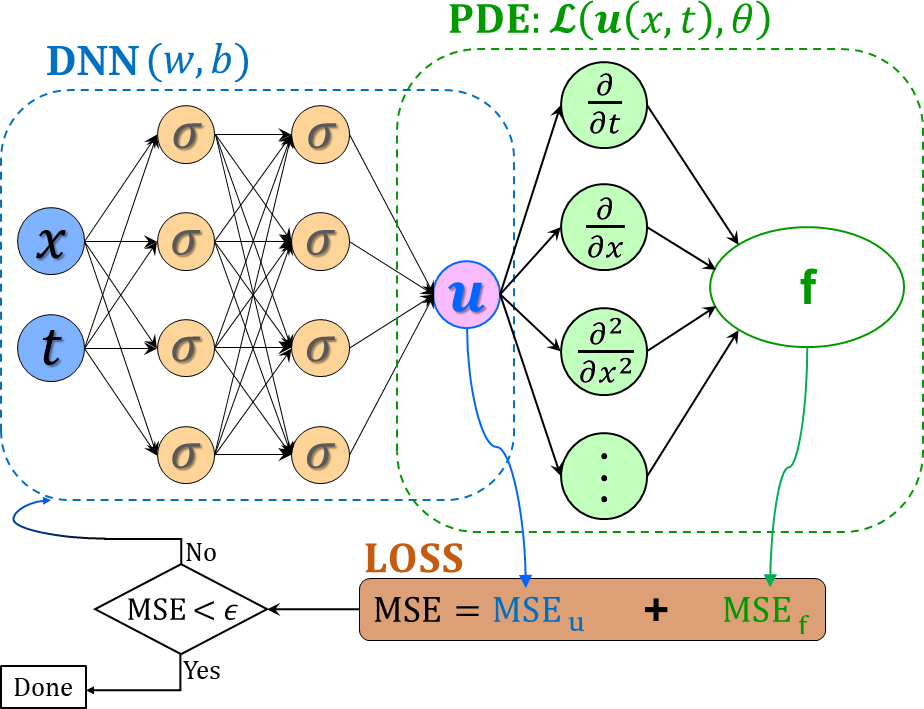
\includegraphics[width=\columnwidth]{nn}
\caption{Schematic showing an example structure and loss function, for the PINN approach. The symbol $\theta$ represents the optimization algorithm. The $\epsilon$ represents the smallest threshold error in the optimization algorithm.\\
Source: Adapted from Meng et al. (2020) \cite{Meng2020}.}
\label{fig:nn}
\end{figure}

According to the work of Raissi et al. (2019) \cite{Raissi2019}, the standard division of the CP dataset into training, validation and testing is not used in this specific PINN model. Instead, a random sample of CPs from the dataset is taken and used to train the PINN. During training, a specific validation set is not used. After training, the network is used to generate two results: ($i$) the discovery of the PDE parameters, and ($ii$) a prediction of the PDE solution.

Once the parameters have been discovered, in a second step, the resulting PINN model is used to predict the velocity field for all points in the defined space and time domain. This predicted velocity field can then be compared with the exact velocity field (generated by GQM), using a relative error to evaluate the accuracy of the prediction, as suggested in Xu et al. (2022) \cite{Xu2022}. Such a relative error is defined by \autoref{eq:error}.

\begin{equation}
R_{L2} = \frac{\| \widehat{U} - U \|}{\|U\|}
\label{eq:error}
\end{equation}

The $\|U\|$ represents the Euclidean L2 norm, which is given by the Euclidean distance from the vector coordinate to the origin of the vector space, i.e. it is the square root of the sum of the squared components of the vector. In the one-dimensional case, the L2 norm is simply given by the value of the velocity.
The $\| \widehat{U} - {U} \| $ represents the application of the L2 norm to the deviation of the estimated velocity field $\widehat{U}$, with respect to the exact velocity field $U$, considering all dataset points in the space and time domains.

The PINN hyperparameters, like the number of hidden layers $N_l(l = 1, 2, ...)$, and the number of neurons in each layer $N_{le}(e = 1, 2, ...)$, can also be optimized by numerical experimentation (trial and error). Optimization of $N_l$ and $N_{le}$, and eventually of other hyperparameters not employed here, is still an unsolved problem, being made empirically \cite{Xu2022}.

As any neural network, PINNs are subjected to overfitting or underfitting. Overfitting means that the DNN performs very well using the training set, but lacks performance using different, new input data of the test set, i.e. it does not generalize. On the other hand, underfitting means that the model performs poorly on both the training and test sets. Obviously, both overfitting and underfitting imply in poor performance of the neural network \cite{Koehrsen2018}.

\subsection{NM-based parameter discovery}
\label{sec:npd}

The inverse problem solved by the implemented PINN to find the coefficients of the differential operators is then compared to the chosen NM-based method, the Sparse Identification of Nonlinear Dynamical Systems (SINDy) method \cite{Boninsegna2018}. This is a method developed for solving the identification problem of dynamical systems, which are systems that change over time. SINDy uses sparse regression to create a linear combination of basis functions to captures the dynamic behavior of the considered physical system. It employs observational or synthetic data to obtain the governing equations that fit such data of the dynamical systems. The discovered equations can then be used to predict future states, inform control inputs, or enable theoretical research using analytical techniques~\cite{Brunton2016}.

Assuming a physical system that evolves in time $t$ and space $x$ defined by a collection of measurements $x(t)\in \mathbb{R}$. Time evolution of $x(t)$ is modeled by SINDy using a nonlinear function $f(x(t))$ (\autoref{eq:sn1}). The vector $x(t)=[x_1(t), x_2(t), \dots x_n(t)]^\top$ represents the state of the physical system at time $t$. The problem solved by SINDy is shown in \autoref{eq:sn2}, where the function $f(x(t))$ is expressed as a matrix $\Theta$ of basis functions applied to the input data $X$, i.e. $\Theta(X)$, which is then multiplied by a matrix $\Xi$ of coefficients that weighs these basis functions. Along the iterations, these coefficients are optimized until achieving convergence by means of an objective function (\autoref{eq:opt}) that assess the correctness of the solution given by [$\Theta(X)\,\Xi$] at a given iteration. It is assumed that $f(x(t))$ is usually sparse in the space of a suitable set of basis functions, i.e. that much of the coefficients of matrix $\Xi$ are zero. 

\begin{equation}
\frac{d}{dt}x(t) = f(x(t))
\label{eq:sn1}\end{equation}

\begin{equation}
\dot{X} \; = \Theta \,(X)\,\,\Xi
\label{eq:sn2}
\end{equation}

SINDy applies a sparsity-promoting regression (such as LASSO \cite{Tibshirani2011}) to a library of nonlinear candidate functions produced from the measurements, but restricting the number of basis functions to obtain a compact representation of the function and avoid overfitting.   
SINDy has been effectively used to solve a variety of problems, including linear and nonlinear oscillators, chaotic systems, and fluid dynamics \cite{Brunton2016}. SINDy is implemented by the sparse regression package PySINDy\footnote{\url{http://pysindy.readthedocs.io}} which includes several implementations for the sparse identification method of nonlinear dynamical systems from various authors, being  comprehensive literature reviews available at \cite{DeSilva2020} and \cite{Kaptanoglu2022}. Part of the code implemented in this work was reused and adapted from PySINDy library examples. PySINDy runs on CPU.


This work employs four of these implementations, known as Sparse Regression Optimizers (SRO), which are part of the parameter discovery package and can be selected separately, producing a result for each choice: Sequentially Threshold Least Squares (STLSQ), Orthogonal Least Squares of Forward Regression (FROLS), Sparse Relaxed Regularized Regression (SR3), and Sparse Stepwise Regression (SSR). To keep things simple, we'll treat each of these as a separate NM.

A code snippet of this framework is shown in \autoref{lst:nm}, where \texttt{optimizer} is the chosen optimization method (exemplified in the code as STLSQ), \texttt{SINDy} defines the model, \texttt{fit} discovers the parameters, and \texttt{print} shows the result. 

\begin{minipage}[htb]{.94\columnwidth}
\begin{lstlisting}[language=Python, label=lst:nm, caption={Python code snippet that implements the NM for data-driven PDE parameter discovery. The STLSQ is one of the optimizers in the PySINDy framework.}]
optimizer = ps.STLSQ(threshold=2, alpha=1e-5, normalize_columns=True)
model = ps.SINDy(feature_library=pde_lib,
                 optimizer=optimizer,
                 feature_names=["u"])
model.fit(u, t=dt)
model.print()
\end{lstlisting}
\end{minipage}%

The dataset used by SINDy for each of the 4 optimizers is the same used in the PINN method, but employing the full dataset instead of the set of CPs. Parameter discovery using PINN required training the network with the set of CPs, use of the Burgers' PDE in the loss function, etc. After training, the predicted velocity field in space and time is then compared to the exact field. In the case of SINDy,
the complete dataset is used to obtain the parameters, with no further comparison \cite{Brunton2016}. However, parameters discovered by PINN and SINDy are compared in order to evaluate the accuracy of both approaches using the coefficients of the known PDE as reference.
Although possible, some optimizations were not made to SINDy in order to obtain better accuracy, being the default settings of the framework used. These possible optimizations can be performed as future work.

Except in the case of SINDy with the SR3 optimizer, the other optimizers employ the objective function that must be minimized, which can be seen in the \autoref{eq:opt}.

\begin{minipage}[htb]{.95\columnwidth}\bigskip\begin{equation}
\| \ y \ - \ X \ w \ \|^2 \ \ + \ \ \alpha \ \| \ w \ \|^2
\label{eq:opt}\end{equation}
Above, $w$ is the weight matrix containing the set of basis functions that maps the dataset contained in $X$ to the solution $y$, i.e. $w$ corresponds to the 2nd member ([$\Theta(X)\,\Xi$]) of \autoref{eq:sn2}, and $\alpha$ is a regularization coefficient applied to $w$, helping prevent overfitting.
\bigskip\end{minipage}%





In order to minimize the objective function, the STLSQ \cite{Brunton2016} algorithm uses ridge regression with sequential threshold, and iteratively runs the least squares algorithm, but masking elements below a specific threshold. The FROLS \cite{Billings2013} algorithm is a greedy algorithm that iteratively selects the most correlated function in the library. The SSR \cite{Boninsegna2018} is also a greedy algorithm that iteratively eliminates the smallest coefficients. A greedy algorithm is any algorithm that uses the heuristic of choosing the locally optimal solution at every iteration \cite{Black2005}. Regardless of not assuredly finding a global optimal solution, greedy heuristics can produce locally optimal solutions that approximate a globally optimal solution in a reasonable amount of time. Along the iterations, the SSR and FROLS algorithms respectively truncate (or add) one nonzero coefficient at each algorithm iteration.

The SR3 algorithm \cite{Champion2019} is a relaxed and sparse regularized regression with linear (dis)equality constraints that attempts to minimize the objective function (\autoref{eq:sr3}).

\begin{minipage}[htb]{.95\columnwidth}\bigskip\begin{equation}\begin{aligned}
&0.5  \|  y  -  X  w \|^2 + \lambda  R(u) + (0.5 / \nu)  \|  w  -  u  \|^2\\
&\text{subject to } Cw = d
\label{eq:sr3}\end{aligned}\end{equation}
over $u$ and $w$, where $R(u)$ is a regularization function, $C$ is a constraint matrix, and $d$ is a vector of values.
\bigskip\end{minipage}%

\subsection{Computing environment}
\label{sec:cenv}

The PINN and the four PySINDy codes\footnote{The codes are available at \url{http://github.com/efurlanm/pd1b24}} were executed in two different computing environments. It is important to note that the PINN model runs on GPU, while PySINDy runs on CPU.

The first environment is a local machine, a PC with a 6-core Intel i7 9750h CPU with 6 cores, 8 GB of main memory, and an NVIDIA GTX 1050 GPU (768 CUDA cores and 3 GB of memory). The second environment is the Santos Dumont (SDumont) supercomputer of the National Scientific Computing Laboratory (LNCC), more specifically a single Bull Sequana X1120 processing node with two 24-core Intel Xeon Gold 6252 Skylake 2.1 GHz processors (total of 48 cores), 384 GB of main memory and four Nvidia Volta V100 GPUs, although only one GPU was employed. Both computing environments included the Python\footnote{\url{http://www.python.org}} 3.7 interpreter and the TensorFlow\footnote{\url{http://www.tensorflow.org}} v1.15 machine learning platform.

\section{Results}
\label{sec:resu}

The results are divided into two parts of experiments: the first one compares the results of PINN with the 4 SINDy versions, and the second evaluates the PINN implementation for various hyperparameters and CP sizes. The first part uses datasets related to different problem sizes ($x$ space versus $t$ time discretization): 128x64, 256x128, and 512x256, while the second part uses only a 256x100 problem size. The GQM is used to generate the dataset corresponding to the exact solution (reference), which are then employed by the SINDy versions, and also to extract the set of CPs used by the PINN implementation. The MLP architecture used for the PINN implementation in the first part has one input layer, 3 hidden layers with 20 neurons each, and one output layer. The PINN undergoes training and PDE parameters are estimated, solving the inverse problem, and the resulting model estimates the solution (space versus time field). The processing-time data obtained in the all experiments is given by the average of 3  executions. 

\subsection{Part I - Comparison of PINN and SINDy for parameter discovery}

Tables \ref{tab:nm-pinn-time-comp-01} and \ref{tab:nm-pinn-time-comp-02} show  the average of elapsed times of 3 runs on the local machine for the PINN (using GPU) and the 4 SINDy implementations (only CPU), for the 3 problem sizes and for the two cases of viscosity.  In the case of PINN, training time to estimate the parameters and prediction time of the resulting 1D field using the trained model are shown. Processing times of SINDy versions are consistently lower than those of the PINN model, even considering that the latter executes using GPU. Therefore, future studies must consider the tradeoff between accuracy and processing times when comparing PINNs and numerical methods like SINDy. 


\begin{table}[htb]\centering
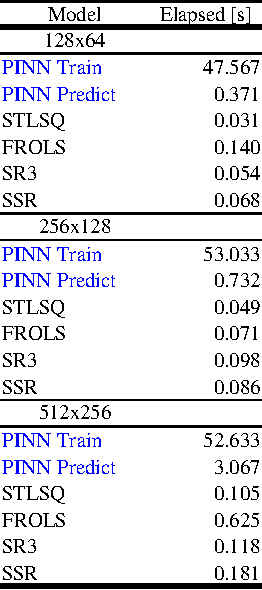
\includegraphics[width=.41\columnwidth]{nm-pinn-time-comp-01}
\caption{Comparison of elapsed times (average of 3 runs) for the PINN and the 4 SINDy models for kinematic viscosity of the fluid of ${0.01}/{\pi}$, and for execution on the local machine (PC).}
\label{tab:nm-pinn-time-comp-01}
\end{table}


\begin{table}[htb]\centering
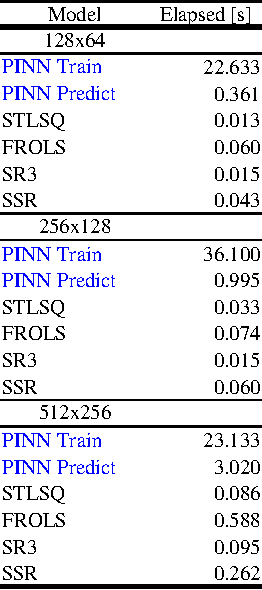
\includegraphics[width=.41\columnwidth]{nm-pinn-time-comp-02}
\caption{Comparison of elapsed times (average of 3 runs) for the PINN and the 4 SINDy models for kinematic viscosity of the fluid of ${0.1}/{\pi}$, and for execution on the local machine (PC).}
\label{tab:nm-pinn-time-comp-02}
\end{table}

Tables \ref{tab:nm-pinn-01} and \ref{tab:nm-pinn-02} show the results obtained for the PDE parameter discovery, comparing the  PINN and the 4 SINDy implementations (STLSQ, FROLS, SR3 and SSR, discussed in \autoref{sec:npd}), and also considering 2 different viscosity values in the 1D Burgers' equation, ${0.01}/{\pi}$ and ${0.1}/{\pi}$. As already commented, 3 sizes of problems are considered: 128x64, 256x128 and 512x256. 

Subscripts denote partial differentiation in time and space, e.g. u\_x denotes ${du}/{dx}$, u\_xx denotes ${d^2u}/{dx^2}$, and so on. 
At the top of each table is shown the \textit{Exact PDE} 1D Burgers' equation (e.g., $u_t + 1.0 u u_x - 0.003183 u_{xx} = 0$) used to generate the datasets.

In the case of PINN, training is done using 2,000 CPs randomly obtained from the dataset, regardless of the size of the problem. 
In the case of SINDy implementations, the complete dataset is used in the model to obtain the parameters. In \ref{tab:nm-pinn-01} the viscosity value (${0.01}/{\pi}$) is lower than in the second (${0.1}/{\pi}$) in order to check if SINDy accuracy is compromised for  small viscosity values, as confirmed by the results. PINN accuracy was good, even using the set of CPs extracted from the smaller dataset, and such accuracy improves with the problem size. \ref{tab:nm-pinn-01} is for experiments with the higher viscosity value, showing that the accuracy of the SINDy implementations improved in comparison to the results of the preceding table, but are still lower than those obtained by PINN.

\begin{table}[htb]\centering
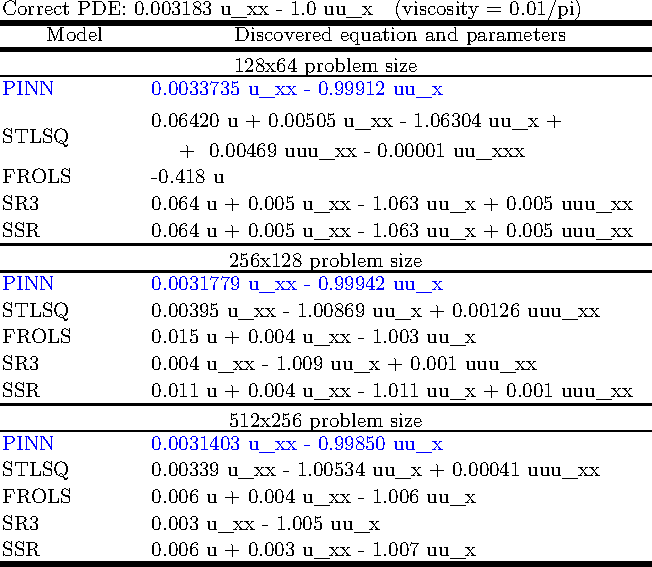
\includegraphics[width=\columnwidth]{nm-pinn-01}
\caption{Comparison of the results of the parameter discovery for the 1D Burgers' equation using PINN (in blue) and the 4 SINDy versions (kinematic viscosity of the fluid of ${0.01}/{\pi}$).}
\label{tab:nm-pinn-01}
\end{table}

\begin{table}[htb]\centering
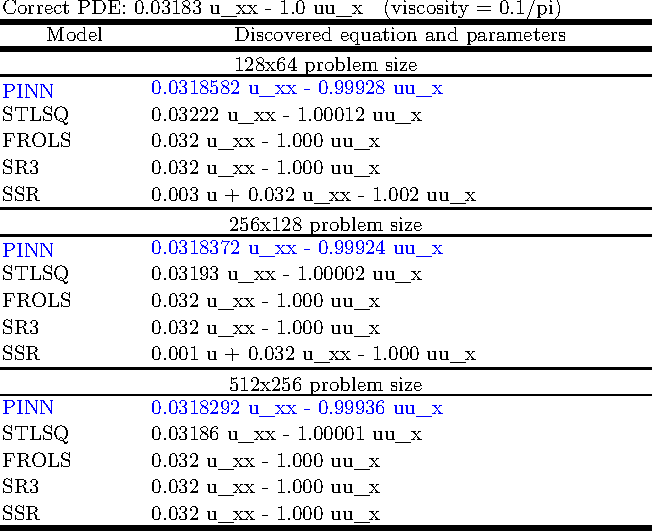
\includegraphics[width=\columnwidth]{nm-pinn-02}
\caption{Comparison of the results of the parameter discovery for the 1D Burgers' equation using PINN (in blue) and the 4 SINDy versions (kinematic viscosity of the fluid of ${0.1}/{\pi}$).}
\label{tab:nm-pinn-02}
\end{table}

 The next subsections present the solution field $u(t,x)$ generated by the PINN implementation for the 3 problem sizes, and for the 2 viscosity values. For each case, there are figures showing the predicted solution $u(t,x)$ with marks representing the CPs, and a particular snapshot at time $t=0.5$ comparing the PINN prediction and the exact solution. These figures allow a visual assessment of the accuracy of the solutions.

\subsubsection{Problem size 128x64}

Figures \ref{fig:pinn-01-128-a}, \ref{fig:pinn-01-128-b}, \ref{fig:pinn-02-128-a}, and \ref{fig:pinn-02-128-b} show, for the problem size 128x64, the solutions for the viscosities ${0.01}/{\pi}$ and ${0.1}/{\pi}$. 
Figures \ref{fig:pinn-01-128-a} and \ref{fig:pinn-02-128-a} show the predicted spatio-temporal solution $u(t, x)$, and the CPs used to training are represented as dark marks on the graph.
Since the dataset is relatively small and the number of CP is 2,000, the small marks are aligned and may not appear random at first. 
At the top and bottom of the figure, ($x=1.0$ and $x=-1.0$), are the CPs related to the boundary conditions (BC) of the PDE, on the left side ($t=0, 0$) are the CPs relative to the initial conditions (IC), and in the center of the figure ($x=0.0$) the complex non-linear behavior (sometimes called formation of a shock wave) of the Burgers' equation with lower viscosity is represented.
The remaining randomly selected CPs appear on the graph. Although it was not done this way, it is possible to select more points in the BC and IC regions to reinforce network training, if necessary.

Figures \ref{fig:pinn-01-128-b} and \ref{fig:pinn-02-128-b} show a snapshot in time comparing the superimposed solution for the PINN method and the exact numerical solution.
It is possible to see that even using a few CPs, the PINN was able to accurately capture the complex non-linear behavior of the Burgers' equation, which presents the formation of an accentuated internal layer around t = 0.4, which is generally difficult to solve with traditional NM and requires a laborious spatio-temporal discretization of the equation. 
In this scenario, we can directly address the nonlinear problem without needing to commit to any prior assumptions, linearization, or local time step.

Due to the number of CPs being constant even when the size of the dataset varies, great variation in the discovery of parameters in the PINN model is not expected. In the case of the NMs seen in Tables \ref{tab:nm-pinn-01} and \ref {tab:nm-pinn-02}, the variation is expected because the NM uses the complete dataset (does not use CP). 
In addition, there is also variation related to each NM algorithm.
For the \autoref{tab:nm-pinn-01} with lower viscosity, it is possible to observe that for 128x64 (total of 8,192 data points) the accuracy of the NM was not good, unlike the PINN model which obtained good accuracy even with a smaller amount (2000 CPs) of training data.
As for \autoref{tab:nm-pinn-02} with higher viscosity, it is possible to observe that for 128x64 the NM showed better accuracy, especially FROLS and SR3, approaching the PINN model.

\begin{figure}[htb]\centering
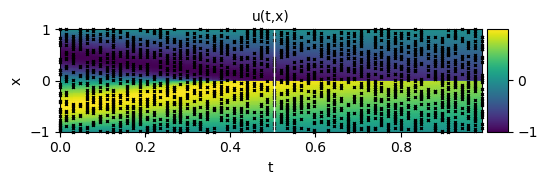
\includegraphics[width=\columnwidth]{pinn-01-128-a}
\caption{PINN predicted solution $u(t, x)$ for viscosity ${0.01}/{\pi}$ and problem size 128x64.}
\label{fig:pinn-01-128-a}
\end{figure}

\begin{figure}[htb]\centering
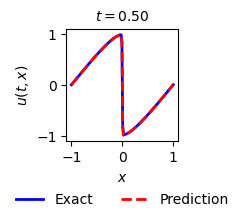
\includegraphics[width=.4\columnwidth]{pinn-01-128-b}
\caption{Comparison of the solutions obtained by PINN (in red) and the exact numerical solution (in blue) for the $t=0.5$ snapshot (viscosity of ${0.01}/{\pi}$ and problem size of 128x64).}
\label{fig:pinn-01-128-b}
\end{figure}

\begin{figure}[htb]\centering
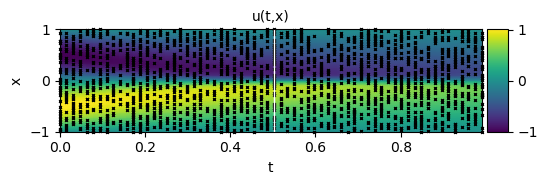
\includegraphics[width=\columnwidth]{pinn-02-128-a}
\caption{PINN predicted solution $u(t, x)$ for viscosity ${0.1}/{\pi}$ and problem size 128x64.}
\label{fig:pinn-02-128-a}
\end{figure}

\begin{figure}[htb]\centering
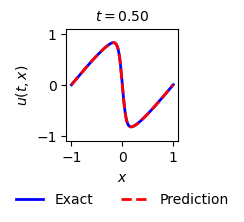
\includegraphics[width=.4\columnwidth]{pinn-02-128-b}
\caption{Comparison of the solutions obtained by PINN (in red) and the exact numerical solution (in blue) for the $t=0.5$ snapshot (viscosity of ${0.1}/{\pi}$ and problem size of 128x64).}
\label{fig:pinn-02-128-b}
\end{figure}

\subsubsection{Problem size 256x128}

The Figures \ref{fig:pinn-01-256-a}, \ref{fig:pinn-01-256-b}, \ref{fig:pinn-02-256-a} and \ref{fig:pinn-02-256-b} show, for the problem size 256x128, the solutions for the viscosities ${0.01}/{\pi}$ and ${0.1}/{\pi}$. 
Much of what was presented in the previous section also applies to this section.
In Figures \ref{fig:pinn-01-256-a} and \ref{fig:pinn-02-256-a} one can initially observe a better distribution of CPs in a more random way, due to the fact that the set of data to be larger and the size of the CP set remains at 2,000 CPs, allowing the CP to be distributed a little better in the graph.
Figures \ref{fig:pinn-01-256-b} and \ref{fig:pinn-02-256-b} show the same behavior as the previous subsection, even because the amount of CP is the same. 
For the \autoref{tab:nm-pinn-01} with lower viscosity, and 256x128 problem size, the NMs were not accurate. For low viscosity, in most cases, regardless of the dataset, the PINN model showed better accuracy. For the \autoref{tab:nm-pinn-02} with higher viscosity, and 256x64 problem size, most of the NMs behaved well, differently from what occurs in the case with lower viscosity.

\begin{figure}[htb]\centering
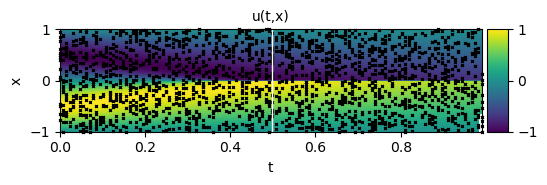
\includegraphics[width=\columnwidth]{pinn-01-256-a}
\caption{PINN predicted solution $u(t, x)$ for viscosity ${0.01}/{\pi}$ and problem size 256x128.}
\label{fig:pinn-01-256-a}
\end{figure}

\begin{figure}[htb]\centering
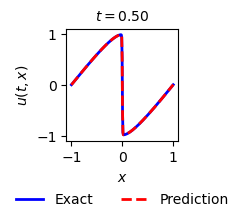
\includegraphics[width=.4\columnwidth]{pinn-01-256-b}
\caption{Comparison of the solutions obtained by PINN (in red) and the exact numerical solution (in blue) for the $t=0.5$ snapshot (viscosity of ${0.01}/{\pi}$ and problem size of 256x128).}
\label{fig:pinn-01-256-b}
\end{figure}

\begin{figure}[htb]\centering
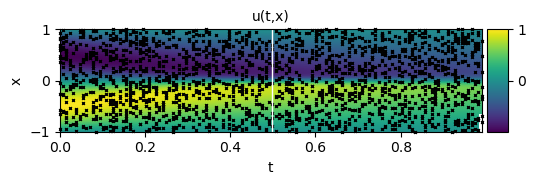
\includegraphics[width=\columnwidth]{pinn-02-256-a}
\caption{PINN predicted solution $u(t, x)$ for viscosity ${0.1}/{\pi}$ and problem size 256x128.}
\label{fig:pinn-02-256-a}
\end{figure}

\begin{figure}[htb]\centering
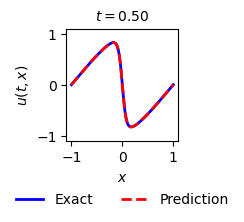
\includegraphics[width=.4\columnwidth]{pinn-02-256-b}
\caption{Comparison of the solutions obtained by PINN (in red) and the exact numerical solution (in blue) for the $t=0.5$ snapshot (viscosity of ${0.1}/{\pi}$ and problem size of 256x128).}
\label{fig:pinn-02-256-b}
\end{figure}

\subsubsection{Problem size 512x256}

The Figures \ref{fig:pinn-01-512-a}, \ref{fig:pinn-01-512-b}, \ref{fig:pinn-02-512-a} and \ref{fig:pinn-02-512-b} show, for the problem size 512x256, the same behavior as the previous subsection.
For Tables \ref{tab:nm-pinn-01} and \ref{tab:nm-pinn-02}, 512x256 problem size, the NMs showed similar behavior to the previous section, with the SSR method standing out.

\begin{figure}[htb]\centering
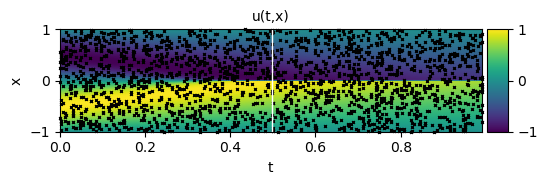
\includegraphics[width=\columnwidth]{pinn-01-512-a}
\caption{PINN predicted solution $u(t, x)$ for viscosity ${0.01}/{\pi}$ and problem size 512x256.}
\label{fig:pinn-01-512-a}
\end{figure}

\begin{figure}[htb]\centering
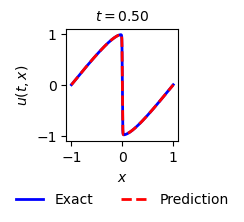
\includegraphics[width=.4\columnwidth]{pinn-01-512-b}
\caption{Comparison of the solutions obtained by PINN (in red) and the exact numerical solution (in blue) for the $t=0.5$ snapshot (viscosity of ${0.01}/{\pi}$ and problem size of 512x256).}
\label{fig:pinn-01-512-b}
\end{figure}

\begin{figure}[htb]\centering
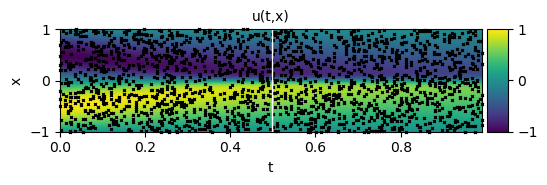
\includegraphics[width=\columnwidth]{pinn-02-512-a}
\caption{PINN predicted solution $u(t, x)$ for viscosity ${0.1}/{\pi}$ and problem size 512x256.}
\label{fig:pinn-02-512-a}
\end{figure}

\begin{figure}[htb]\centering
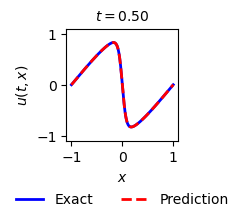
\includegraphics[width=.4\columnwidth]{pinn-02-512-b}
\caption{Comparison of the solutions obtained by PINN (in red) and the exact numerical solution (in blue) for the $t=0.5$ snapshot (viscosity of ${0.1}/{\pi}$ and problem size of 512x256).}
\label{fig:pinn-02-512-b}
\end{figure}


\subsection{Part II - Evaluation of PINN according to hyperparameter set and size of CP set}

PINN processing time and accuracy is evaluated using the model generated with different sets of hyperparameters and CP set sizes in experiments executed on SDumont. Resulting predicted 1D fields are presented in figures, which are similar to those of the previous section.
Following, PINN accuracy and processing times are evaluated as a function of the number of neurons per hidden layer, the number of hidden layers, and also the size of the CP set.

\subsubsection{Visual assessment of PINN}

In this section, the network architecture is the same employed for the preceding comparisons between PINN and SINDy implementations (single input and output layers and 4 hidden layers with 20 neurons each).
A visual assessment of predictive accuracy for problem size 256x100 and fluid viscosity of 0.01 is shown in \autoref{fig:bur1}, with time $t$ on the horizontal axis and spatial coordinate $x$ on the vertical axis. The color scale refers to the velocity $u(t, x)$. The black dots on the graph represent the 2,000 CPs randomly generated from the dataset and used for training.  \autoref {fig:bur2} shows a specific snapshot at $t=0.5$, where it is possible to observe the overlapping solutions for PINN and GQM (exact).  For this specific result, the equation obtained by PINN is $u_t + 0.99967 u u_x - 0.0030988 u_{xx} = 0$, while the exact PDE is $u_t + u u_x - 0 ,0031831 u_{xx} = 0$. Thus, the PINN could identify the underlying PDE with good accuracy.

\begin{figure}[htb]\centering
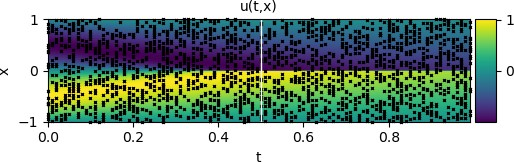
\includegraphics[width=\columnwidth]{burg-01.jpg}
\caption{PINN predicted solution $u(t, x)$ for viscosity ${0.01}/{\pi}$ and problem size 256x100 (black dots denote the 2,000 randomly assigned CPs).} 
\label{fig:bur1}
\end{figure}

\begin{figure}[htb]\centering
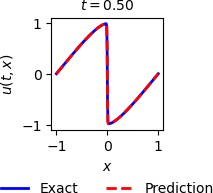
\includegraphics[width=.4\columnwidth]{burg-02.jpg}
\caption{Comparison of the solutions obtained by PINN (in red) and the exact numerical solution (in blue) for the $t=0.5$ snapshot (viscosity of ${0.01}/{\pi}$ and problem size of 256x100).}
\label{fig:bur2}
\end{figure}

\subsubsection{Influence of PINN Number of Layers and of Neurons}

For the results presented below, the hyperparameters $N_{l}$ (number of hidden layers) and $N_{le}$ (number of neurons per hidden layer) were varied, as well as the number of CPs for training.
The \autoref{tab:resu1} shows the relative L2 errors and training times of the PINN, for different hyperparameters used: 10, 15, 20, 25, and 30 neurons per hidden layer, and 1, 2, 4, 6, and 8 hidden layers.
The number of CPs was set at 2,000.
All values shown here are the average of 3 runs.
In this table it is possible to observe that there is a tendency for the best values to be concentrated in the center, probably because there is a problem of underfitting or overfitting in the values at the edges of the table. For future work, it would be interesting to better evaluate this behavior. One of the highlights is that the smallest error is obtained with 6 hidden layers, not 8. In this specific case, increasing the number of layers not only does not increase accuracy, it also worsens performance.

The \autoref{fig:rlaygrapherror2} shows that the error for 1 hidden layer is high compared to the other number of layers. For 2 layers, there is a significant improvement in accuracy. For 4, 6, and 8 the gain in precision is not that great, but the curves are similar and are in the region of greater accuracy, showing that they would be the best choices.

The \autoref{fig:rlaygraptime2} shows, for 4 hidden layers, a tendency to describe a curve that resembles a parabolic, with a minimum processing time of 20 neurons per hidden layer. This is probably due to the problem of underfitting and overfitting occurring at the beginning and at the end of the curve. Once again, for future work, it would be interesting to better evaluate this behavior.

\begin{table}[htb]\centering
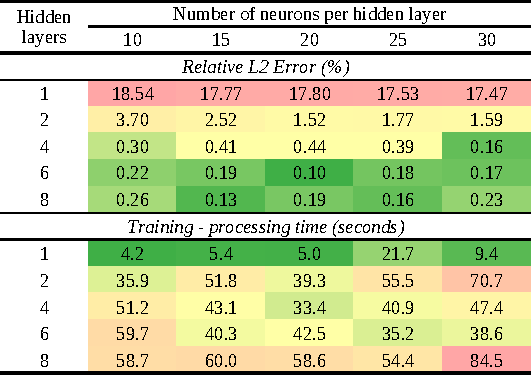
\includegraphics[width=.98\columnwidth]{rlay}
\caption{Relative L2 errors and DNN training times for different number of neurons and hidden layers. On the color scale, the best values are highlighted in green. The simulation ran on the SDumont.}
\label{tab:resu1}
\end{table}

\begin{figure}[htb]\centering
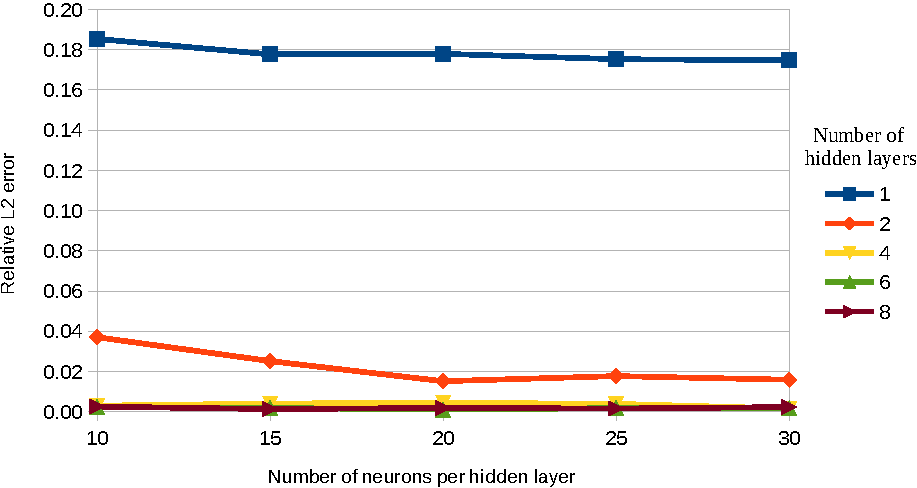
\includegraphics[width=\columnwidth]{rlaygrapherror2}
\caption{Relative L2 error (\%) in function of number of neurons and hidden layers. The simulation ran on the SDumont.}
\label{fig:rlaygrapherror2}
\end{figure}

\begin{figure}[htb]\centering
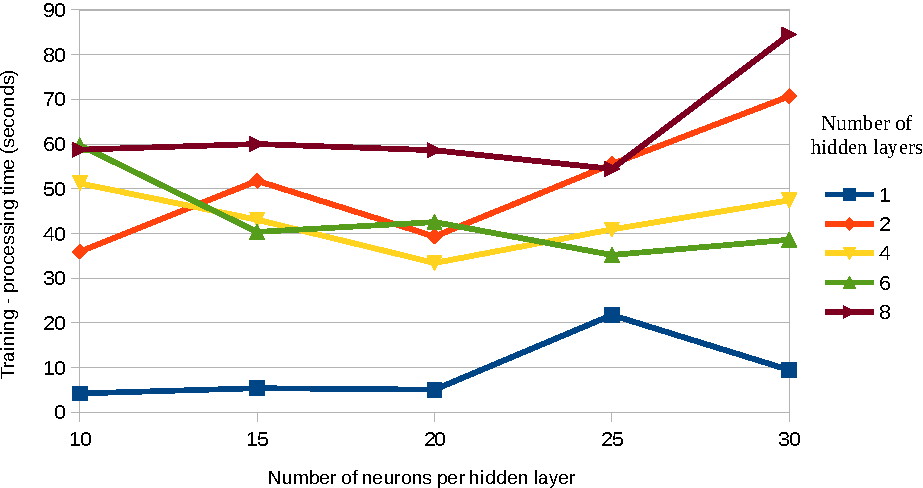
\includegraphics[width=\columnwidth]{rlaygraphtime2}
\caption{Processing times (seconds) in function of number of neurons and hidden layers. The simulation ran on the SDumont.}
\label{fig:rlaygraptime2}
\end{figure}

\subsubsection{Influence of PINN Number of Neurons and Size of CP Set}

The \autoref{tab:rnu8} shows the relative L2 errors and training times of the PINN, for different hyperparameters and number of CP: 10, 15, 20, 25, and 30 neurons per hidden layer, and 400, 800, 1200, 1600, and 2000 CP. The number of layers was set at 8. All values shown here are the average of 3 runs. In this table, as in the previous one, it is possible to observe that there is a tendency for the best values to be concentrated in the center, probably because the problem of underfitting or overfitting is occurring in the values at the edges of the table. Once again, for future work, it would be interesting to better evaluate this behavior. One of the highlights is that considering the smallest error and the shortest processing time, the best dataset size is 1600, and the best number of neurons per hidden layer is 20.

The \autoref{fig:rnu8graphtime2} shows for most curves a tendency to describe a curve that resembles a parabolic, probably due to the problem of underfitting and overfitting occurring at the beginning and end of the curve. Once again, for future work, it would be interesting to better evaluate this behavior. The shortest processing time occurs for 15 neurons per hidden layer, and 1600 CPs.

The \autoref{fig:rnu8grapherror2} shows that the error for 400 CPs is high compared to the others. 800 CPs presents a significant improvement in accuracy, and the other curves are relatively close, not presenting such a relative large accuracy gain.

\begin{table}[htb]\centering
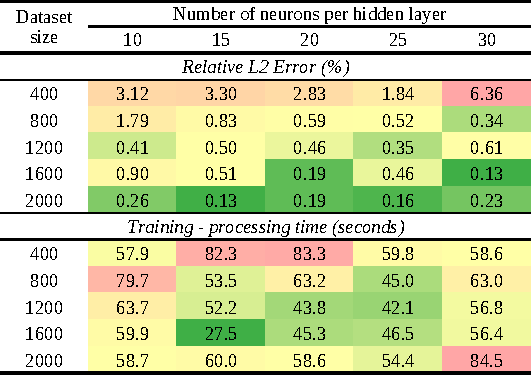
\includegraphics[width=.98\columnwidth]{rnu8}
\caption{Relative L2 errors and DNN training times for different number of neurons and dataset size. The number of hidden layers is set to 8. On the color scale, the best values are highlighted in green. The simulation ran on the SDumont.}
\label{tab:rnu8}
\end{table}

\begin{figure}[htb]\centering
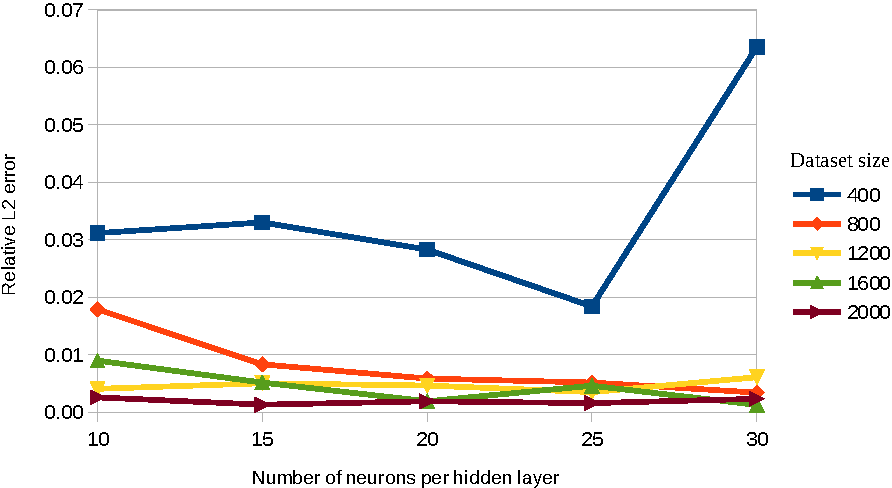
\includegraphics[width=\columnwidth]{rnu8grapherror2.pdf}
\caption{Relative L2 error (\%) in function of number of neurons and dataset size. The number of hidden layers is set to 8. The simulation ran on the SDumont.}
\label{fig:rnu8grapherror2}
\end{figure}

\begin{figure}[htb]\centering
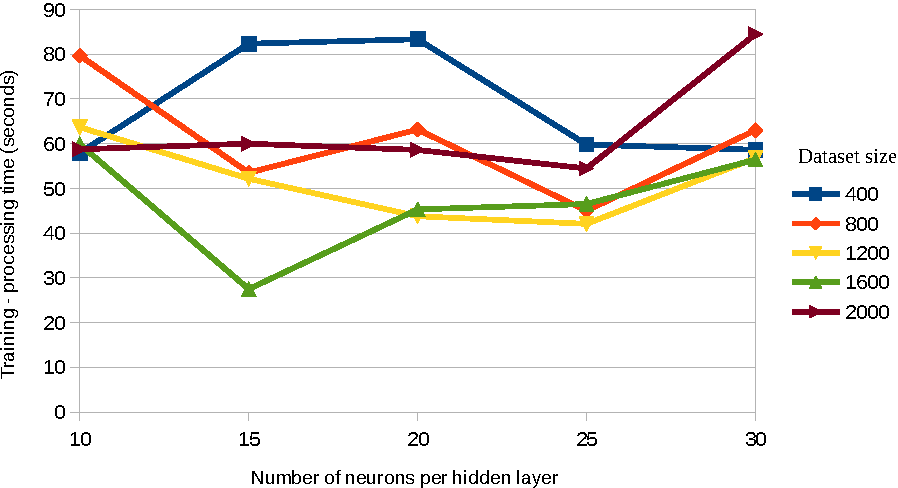
\includegraphics[width=\columnwidth]{rnu8graphtime2.pdf}
\caption{Processing times (seconds) in function of number of neurons and dataset size. The number of hidden layers is set to 8. The simulation ran on the SDumont.}
\label{fig:rnu8graphtime2}
\end{figure}

\subsubsection{PINN Prediction Times}

\autoref{tab:rpre} shows the prediction times of the trained PINN model in function of different number of hidden layers (1, 4, 8) and different numbers of neurons per hidden layer (10, 20, 30). As expected, such times are very close, differently from the corresponding training times, which are higher and differ too much. For instance,  in the case of 4 hidden layers and 20 neurons per layer, training time was 33.4 s, while prediction time was only 0.724 s, or 2.2\%. This is a common issue with neural networks, showing the convenience of avoiding re-training the network whenever possible.


\begin{table}[htb]\centering
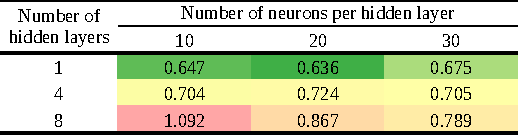
\includegraphics[width=.98\columnwidth]{rpre}
\caption{Prediction times for different number of neurons and hidden layers. On the color scale, the best values are highlighted in green. The simulation ran on the SDumont.}
\label{tab:rpre}
\end{table}



\section{Conclusions}
\label{sec:conc}

Physics-Informed Neural Networks (PINNs) are a novel approach that combines data-driven and physics-based strategies. This work evaluated the inverse problem of data-driven discovery of PDE parameters using PINN and also a NM-based method for a given toy problem, the 1D Burgers equation. This equation models the velocity of a fluid along space and time. In addition, an evaluation was made of the PINN performance in terms of accuracy and processing times considering different MLP hyperparameters and CP set sizes. Adjustment of these characteristics was performed by trial-and-error and indicated an optimal performance range of number of neurons per hidden layer, number of hidden layers, and size of the CP set.

Experiments were performed using different sizes of CP datasets for two different values of viscosity in the Burgers equation. It was shown that the PINN model, even trained with the relatively small subset of CPs achieved good accuracy, compared to the 4 SINDy versions, which employ the entire dataset. Therefore, for the considered test case, the PINN accurately reproduced the complex non-linear behavior of the Burgers' equation.

It was observed that the lowest viscosity value implied in the sharp discontinuities, associated with the formation of a shock wave, which was better modeled by the PINN than by SINDy. Considering the high-viscosity case, SINDy accuracy increased, but PINN accuracy was similar. However, in terms of execution times, SINDy versions were always faster, since the PINN implementation requires training.


As future work, it is proposed to explore other recent PINN-based approaches and/or implementations, as well as use other test cases involving direct and inverse problems associated to PDEs. Real world problems with limited-size or noisy datasets may also be focused. Another work would be to optimize the weather forecast model of the European Centre for Medium-Range Weather Forecasts (ECMWF) by means of developing a PINN-based version of its radiative module ecRad. This is a processing-demanding module that cannot be executed at every timestep of the ECMWF model. In addition, new frameworks and/or libraries for HPC can also be explored for CPU and GPU execution on the LNCC Santos Dumont supercomputer. Among these tools, there is the NVIDIA Modulus\footnote{\url{https://developer.nvidia.com/modulus}} which is a framework for building, training and fine-tuning PINN models. There is also the Horovod\footnote{\url{https://horovod.readthedocs.io}} framework, developed by Uber to improve training using GPUs in MPI parallelization, which enables distributed training using TensorFlow, Keras PyTorch, and Apache MXNet.

\section*{Acknowledgment}

Authors thank LNCC (National Laboratory for Scientific Computing) for grant 205341 AMPEMI (call 2020-I), which allows access to the Santos Dumont supercomputer (node of the SINAPAD, the Brazilian HPC system). This study was financed in part by the Coordination for the Improvement of Higher Education Personnel (CAPES), Brazil, finance Code 001, and also by the CNPq Project 446053/2023-6. The authors also thank the Brazilian Ministry of Science, Technology and Innovation, and the Brazilian Space Agency.


\bibliographystyle{IEEEtran}
\bibliography{library}

\end{document}
